\documentclass[11pt]{article}
\usepackage[T1]{fontenc}
\usepackage{titling}
\usepackage{enumitem}
\usepackage{xcolor}
\usepackage{cite}
\usepackage{amsmath, amsfonts, amssymb, amsthm,tikz}
\usepackage[a4paper, total={6.6in, 8.7in}]{geometry}
\usepackage{fancyhdr}
\usepackage{parskip}
\usepackage{float}
\usepackage{caption}
\usepackage{subcaption}
\usepackage{mathtools}
\usepackage{cancel}
\setenumerate[1]{label=(\arabic*)}
\renewcommand{\qedsymbol}{$\blacksquare$}
\renewcommand{\implies}{\Rightarrow}
\newcommand\cc{\mathcal}
\newcommand\bb{\mathbb}
\newcommand\bbcdot{\boldsymbol{\cdot}}
\newcommand\inv[1]{#1^{-1}}
\newcommand\todo[1]{\color{red} \textbf{TODO: } #1 \color{black}}
\newcommand\hint[1]{\color{blue} \textit{HINT: #1} \color{black}}
\newcommand\cl{\overline}
\newcommand\D{\partial}
\DeclareMathOperator{\Tr}{Tr}
\DeclareMathOperator{\Id}{Id}
\DeclareMathOperator{\Sp}{span}
\DeclareMathOperator{\Ker}{Ker}
\DeclareMathOperator{\Ran}{Ran}
\DeclareMathOperator{\argmax}{argmax}
\DeclareMathOperator{\ImPart}{Im}
\DeclareMathOperator{\Span}{span}
\DeclareMathOperator{\RePart}{Re}
\DeclareMathOperator{\Arg}{Arg}
\DeclareMathOperator{\supp}{supp}
\DeclareMathOperator{\Image}{Image}
\pagestyle{fancy}
\fancyhf{}
\fancyhead[RO]{}
\fancyhead[LO]{}
\fancyfoot[RO]{Page \thepage}
\renewcommand{\headrulewidth}{1pt}
\renewcommand{\footrulewidth}{1pt}
\setlength{\headheight}{13.6pt}
\newtheorem{lemma}{Lemma}
\newtheorem{theorem}{Theorem}
\setlength{\droptitle}{-10em}
% \usepackage{sfmath}
% \renewcommand{\familydefault}{\sfdefault}
% \usepackage{mathpazo}
% \usepackage{palatino}
\usepackage{lmodern}
\title{CBO + BFF applied to Q-control}
\author{Francesco Insulla}
\begin{document}
\maketitle

\section{Introduction}

\section{Models}

Bellman Residual Method (BRM)
\begin{align*}
    J(\theta) &= \mathbb E[((\mathbb T^{\pi_*}-\mathbb I) Q^*(s,a;\theta))^2]\\
&= \mathbb E[\mathbb E[j^{ctrl}(s_m, a_m, s_{m+1};\theta)|s_m,a_m]^2]\\
j^{\text{ctrl}}(s_m, a_m, s_{m+1};\theta) &= r(s_{m+1}, s_m, a_m)  + \gamma \max_{a'} Q^*(s_{m+1},a';\theta) - Q^*(s_m,a_m;\theta)
\end{align*}

Using Batches, and a specific sampling method (UR, DS, BFF), at each
iteration we get an estimate $\tilde J(\theta) $for the loss
$J(\theta)$.

SGD

\begin{align*}
    &M = 1000 && \text{Batch size}\\
    &\text{epochs} = 1 &&\\
    &\gamma = 0.9 && \text{Discount factor}\\
    &\tau_k = \max(\tau_i\cdot \tau_r^k, \tau_i\cdot\tau_f) && \text{Learning rate}
\end{align*}

\begin{align*}
    \Delta\theta_k = -\tau_k \nabla_\theta \tilde J(\theta)
\end{align*}


CBO
\begin{align*}
&N = 90 && \text{Number of particles}\\
&m = 1000 && \text{Batch size}\\
&\text{epochs} = 1 \\
&\gamma = 0.9 && \text{Discount factor}\\
&\delta = 1\times 10^{-5} && \text{Threshold of difference below which particles take a brownian motion step}\\
&\eta_k = \max(\eta_i\cdot \eta_r^k,\eta_i\cdot \eta_f) && \text{Learning rate}\\
&\tau_k =  \max(\tau_i\cdot \tau_r^k,\tau_i\cdot\tau_f) && \text{Exploration rate}\\
&\beta_k =  \min(\beta_i\cdot \beta_r^k,\beta_i\cdot \beta_f) && \text{1/Characteristic energy}
\end{align*}

\begin{align*}
    \bar\theta_k &= \frac{\sum_{j=1}^N \theta_k^{j} \exp(-\beta_k\tilde J(\theta))}{\sum_{j=1}^N  \exp(-\beta_k\tilde J(\theta))}\\
    \Delta \theta^{j}_k &= (-\eta_k I+\tau_k\sqrt{\eta_k}\cdot Z)(\theta^j-\bar\theta); \quad Z=\text{diag}(\{z_i\sim \mathcal N(0,1)\}_{i=1}^N)
\end{align*}
\section{Numerical Example}
\subsection{Setup}
Continuous statespace.
\begin{align*}
    &\mathbb S = (0, 2\pi]\\
    &\Delta s_{m} = a_m\epsilon + \sigma \sqrt{\epsilon} Z_m\\
    &a_m \in\mathbb A = \{\pm 1\}\\
    &a_m\sim \pi_b(\cdot|s_m)\\
    &\varepsilon = \tfrac{2\pi}{32}\\
    &\sigma = 0.2\\
    &r(s_{m+1},s_{m},a_m) = \sin(s_{m+1})+1\\
    &\pi_b(a|s)=\tfrac{1}{|\mathbb A|}\\
    &\text{Model : ResNet}
\end{align*}


Discrete statespace
\begin{align*}
    &\mathbb S = \{\tfrac{2\pi k }{n}: k\in \mathbb Z \cap [0,n-1]\}\\
    &\Delta s_{m} = \tfrac{2\pi}{n}a_m\epsilon + \sigma \sqrt{\epsilon} Z_m\\
    &a_m \in\mathbb A = \{\pm 1\}\\
    &a_m\sim \pi_b(\cdot|s_m)\\
    & n=32\\
    &\varepsilon = 1\\
    &\sigma = 1\\
    &r(s_{m+1},s_{m},a_m) = \sin(s_{m+1})+1\\
    &\pi_b(a|s)=\tfrac{1}{2}+ a\sin(s)\\
    &\text{Model : Tabular}
\end{align*}

\begin{itemize}
    \item
      Policy is sampled using fixed behaviour policy
      $\pi_b:\mathbb A\times \mathbb S\rightarrow[0,1]$ generating long
      and normal trajectories.
    \item
      Reference $\theta^*$ is computed by running UR SGD for 1 epoch based
      on longer trajectory with $\tau=\max(0.8\cdot 0.9992^k, 0.3),$
      $M=1000$.
    \item
      Perform hyperparameter optimization, using optuna, fixing
      $M=1000, \delta = 10^{-5}$, running 150 trials, and $90$ particles
      for CBO, taking error of UR as loss. $3$ Variables for SGD, $9$
      for CBO.
    \item
      Average $10$ instances using best hyperparameters found,
      $\hat\theta$, plotting $Q(\cdot,\cdot;\theta)$, and
      $e_k=e(\theta_k)=\|Q(\cdot, \cdot;\theta^*)-Q(\cdot, \cdot;\theta_k)\|$.
    \item
      Visualize optimization landscape by evaluating error on affine
      combination of parameters of $\theta^*$ and random initialization
      parameters ($e(\alpha\theta^*+(1-\alpha)\theta)$ vs
      $\alpha\in[0,1]$) \emph{since $e$ is a sort of ``distance'', then
      we expect it to be linear near $\alpha=1$}
 \end{itemize}


\subsection{Results}

Continuous

\begin{figure}[h!]
    \centering
    \begin{subfigure}{.9\textwidth}
      \centering
      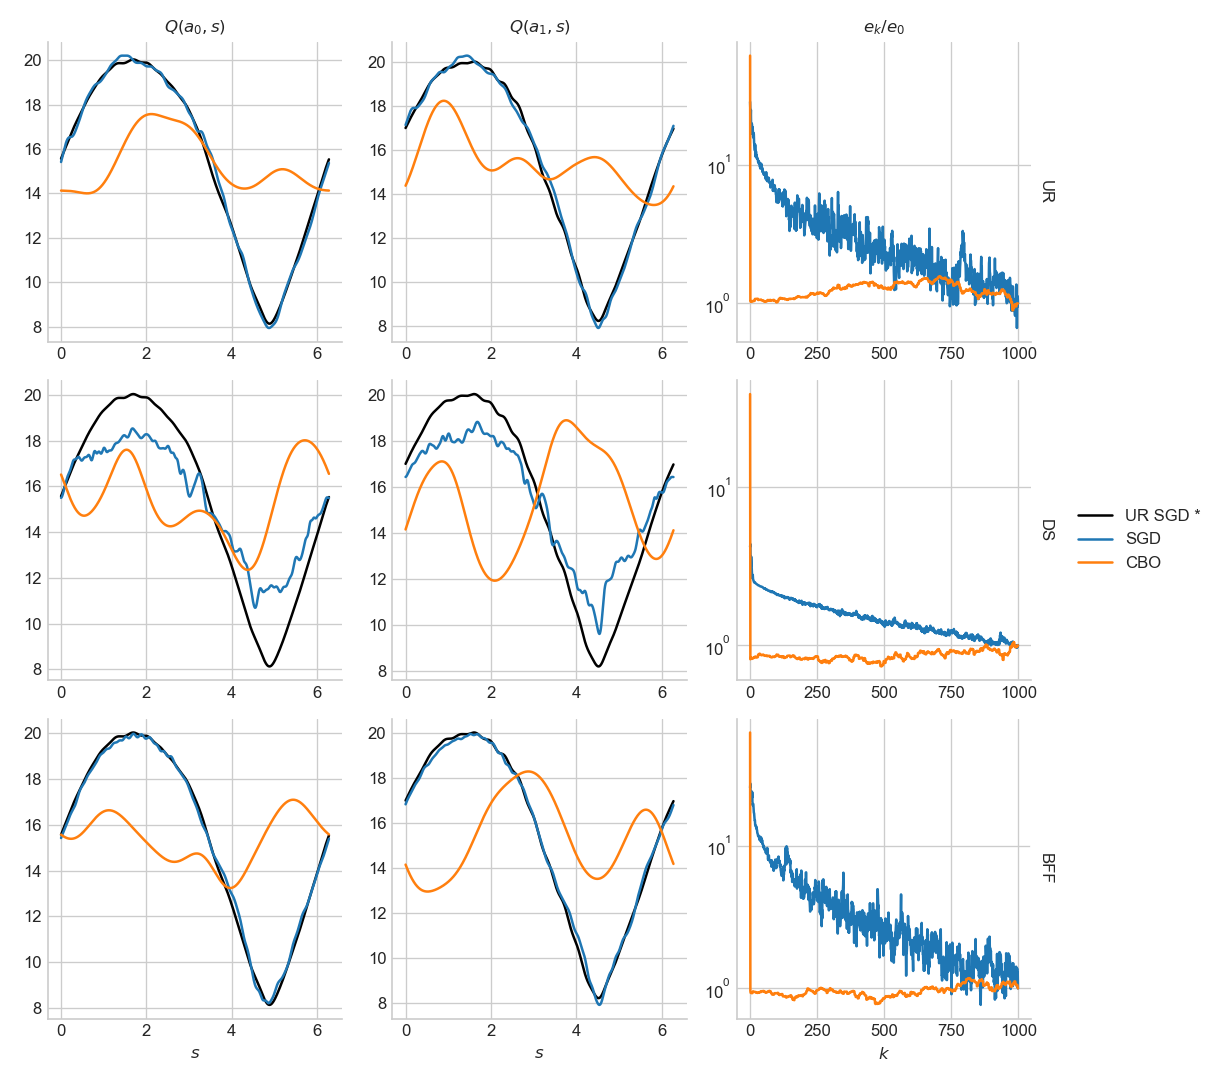
\includegraphics[width=\linewidth]{../figs/Q_ctrl_SGD_vs_CBO_summary_continuous_resnet.png}
      \caption{Summary}
      \label{fig:summary_cont}
    \end{subfigure}
    \begin{subfigure}{.5\textwidth}
      \centering
      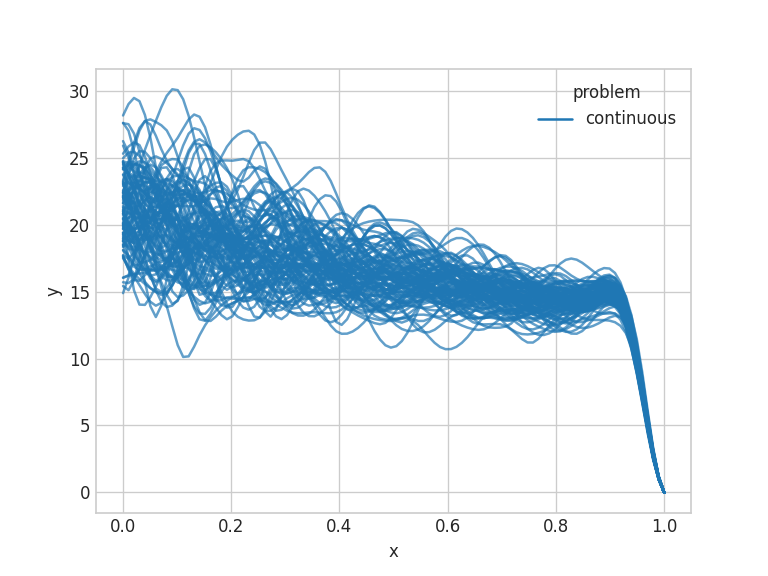
\includegraphics[width=\linewidth]{../figs/Q_ctrl_landscape_plot_continuous_resnet.png}
      \caption{Error landscape}
      \label{fig:error_landscape_cont}
    \end{subfigure}
    \caption{Continuous case}
    \label{fig:cont}
\end{figure}


\begin{tabular}[]{@{}ll@{}}
    SGD & $\tau$\\
    i & 0.08001579582322532\\
    f & 0.9835361410049764\\
    r & 0.950886309322411
\end{tabular}

\begin{tabular}[]{@{}llll@{}}
    CBO & $\eta$ & $\tau$ & $\beta$\\
    i & 0.27998130431694734 & 0.45180905444083275 &
    8.51669145194007\\
    f & 0.5194195083343263 & 0.4287097014952387 &
    1.7500535407136808\\
    r & 0.9698276350455655 & 0.9578569049519733 &
    1.0213109427307054
\end{tabular}


Discrete

\begin{figure}[h!]
    \centering
    \begin{subfigure}{.9\textwidth}
      \centering
      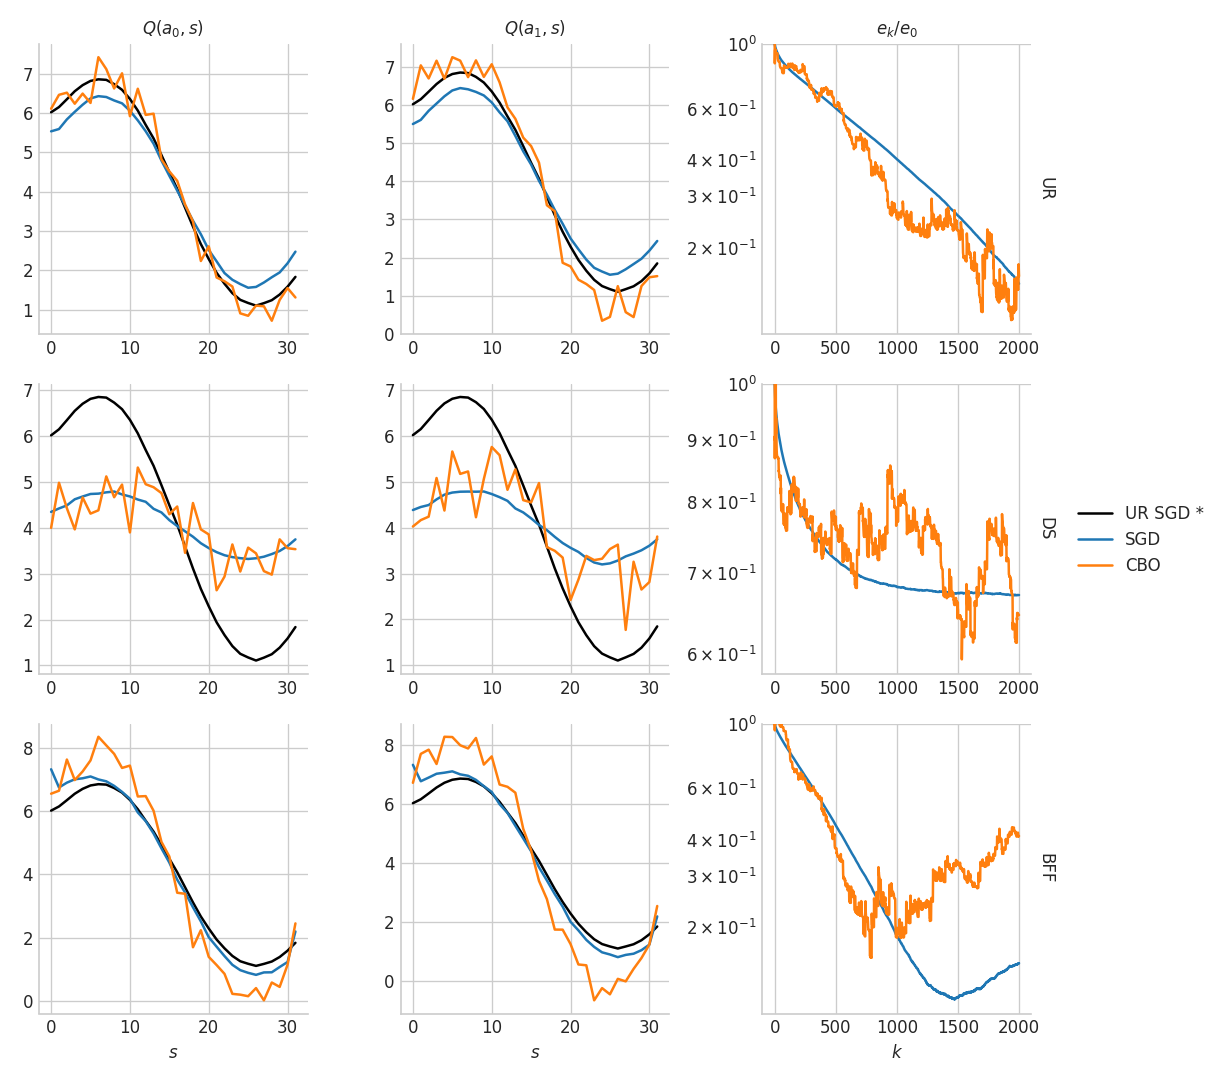
\includegraphics[width=\linewidth]{../figs/Q_ctrl_SGD_vs_CBO_summary_discrete_tabular.png}
      \caption{Summary}
      \label{fig:summary_disc}
    \end{subfigure}
    \begin{subfigure}{.5\textwidth}
      \centering
      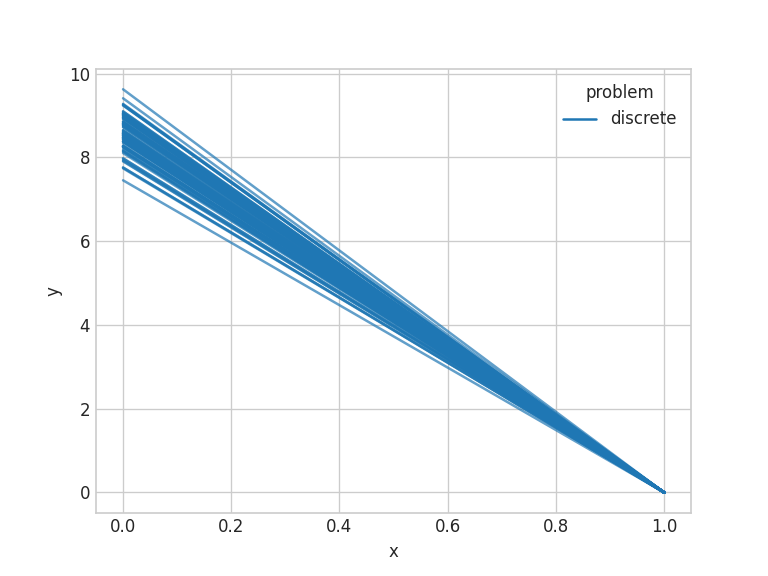
\includegraphics[width=\linewidth]{../figs/Q_ctrl_landscape_plot_discrete_tabular.png}
      \caption{Error landscape}
      \label{fig:error_landscape_disc}
    \end{subfigure}
    \caption{Discrete case}
    \label{fig:disc}
\end{figure}

\begin{tabular}[]{@{}ll@{}}
SGD & $\tau$\\
i & 4.703979337147098\\
f & 0.654883440315296\\
r & 0.9730502549231891
\end{tabular}

\begin{tabular}[]{@{}llll@{}}
CBO & $\eta$ & $\tau$ & $\beta$\\
i & 0.9785432879550536 & 0.893733865582011 &
12.055703082474112\\
f & 0.8242055859864529 & 0.3129317992204857 &
2.6535471522264684\\
r & 0.9827373829994701 & 0.9999130685913801 &
1.019158705231164
\end{tabular}


\section{Conclusion}

An important note is that the differences noted above could be related
to the number of variables in the hyper-parameter search (3 for SGD, 9
for CBO), as well as the complexity/convexity of the problem, ie. if we
performed more trials, it might be possible for CBO $>$ SGD
and BFF $>$ UR in the continuous case, although we have not
observed this fact. This is also based on the fact that CBO
$>$ SGD for V-eval without hyperparameter search.

\end{document}